\subsection{Standard Model W$\gamma$ Production}

A $W$ boson in proton-proton collisions can be produced in the processes $q {\bar{q'}} \rightarrow W$ where $q$ and $\bar{q'}$ are a quark and an antiquark which have a total charge of $+1$ if producing a $W^+$ boson or of $-1$ if producing a $W^-$ boson. The processes $u\bar{d}\rightarrow W^+$ and $d\bar{u}\rightarrow W^-$ are the most likely to occur because $u$ and $d$ are valence quarks in a proton. Antiquarks $\bar{d}$ and $\bar{u}$ come from sea $q\bar{q}$ pairs of the other proton.\\

Decay modes of a $W$ boson include $W^\pm \rightarrow l^\pm \nu_l ({\bar{\nu_l}})$ where $l^\pm=e^\pm$, $\mu^\pm$ or $\tau^\pm$ with branching fractions of ~11\% per a leptonic channel \cite{ref_PDG}. The rest 67\% stands for various $W\rightarrow q\bar{q'}$ decays. In this dissertation we only consider $W^\pm \rightarrow \mu^\pm \nu_\mu ({\bar{\nu_\mu}})$ and $W^\pm \rightarrow e^\pm \nu_e ({\bar{\nu_e}})$ as the cleanest channels.\\

Mass of a $W$ boson $M_W=80$ GeV is much larger than masses of its decay products: $M_\mu=105$ MeV, $M_e=0.5$ MeV, $M_\nu<2$ eV. Therefore, almost all mass of a $W$ boson converts to the kinetic energy of the muon or electron and neutrino or antineutrino.\\

A photon can be emitted from any charged particle of the process: a quark, an antiquark, a charged lepton or a $W$ boson (Fig. \ref{fig:feynmWg_LO_NLO}, top). A quark and an antiquark are initial state particles and, therefore, if one of them radiates a photon, we call such process the Initial State Radiation (ISR). A muon or an electron is a final state particle and if it radiates a photon, we call such process the Final State Radiation (FSR). Finally, a $W$ boson is a gauge boson and if it radiates a photon, the process has a vertex with three gauge bosons: $WW\gamma$, and we call such process the Triple Gauge Coupling (TGC).\\

\begin{figure}[htb]
  \begin{center}
    {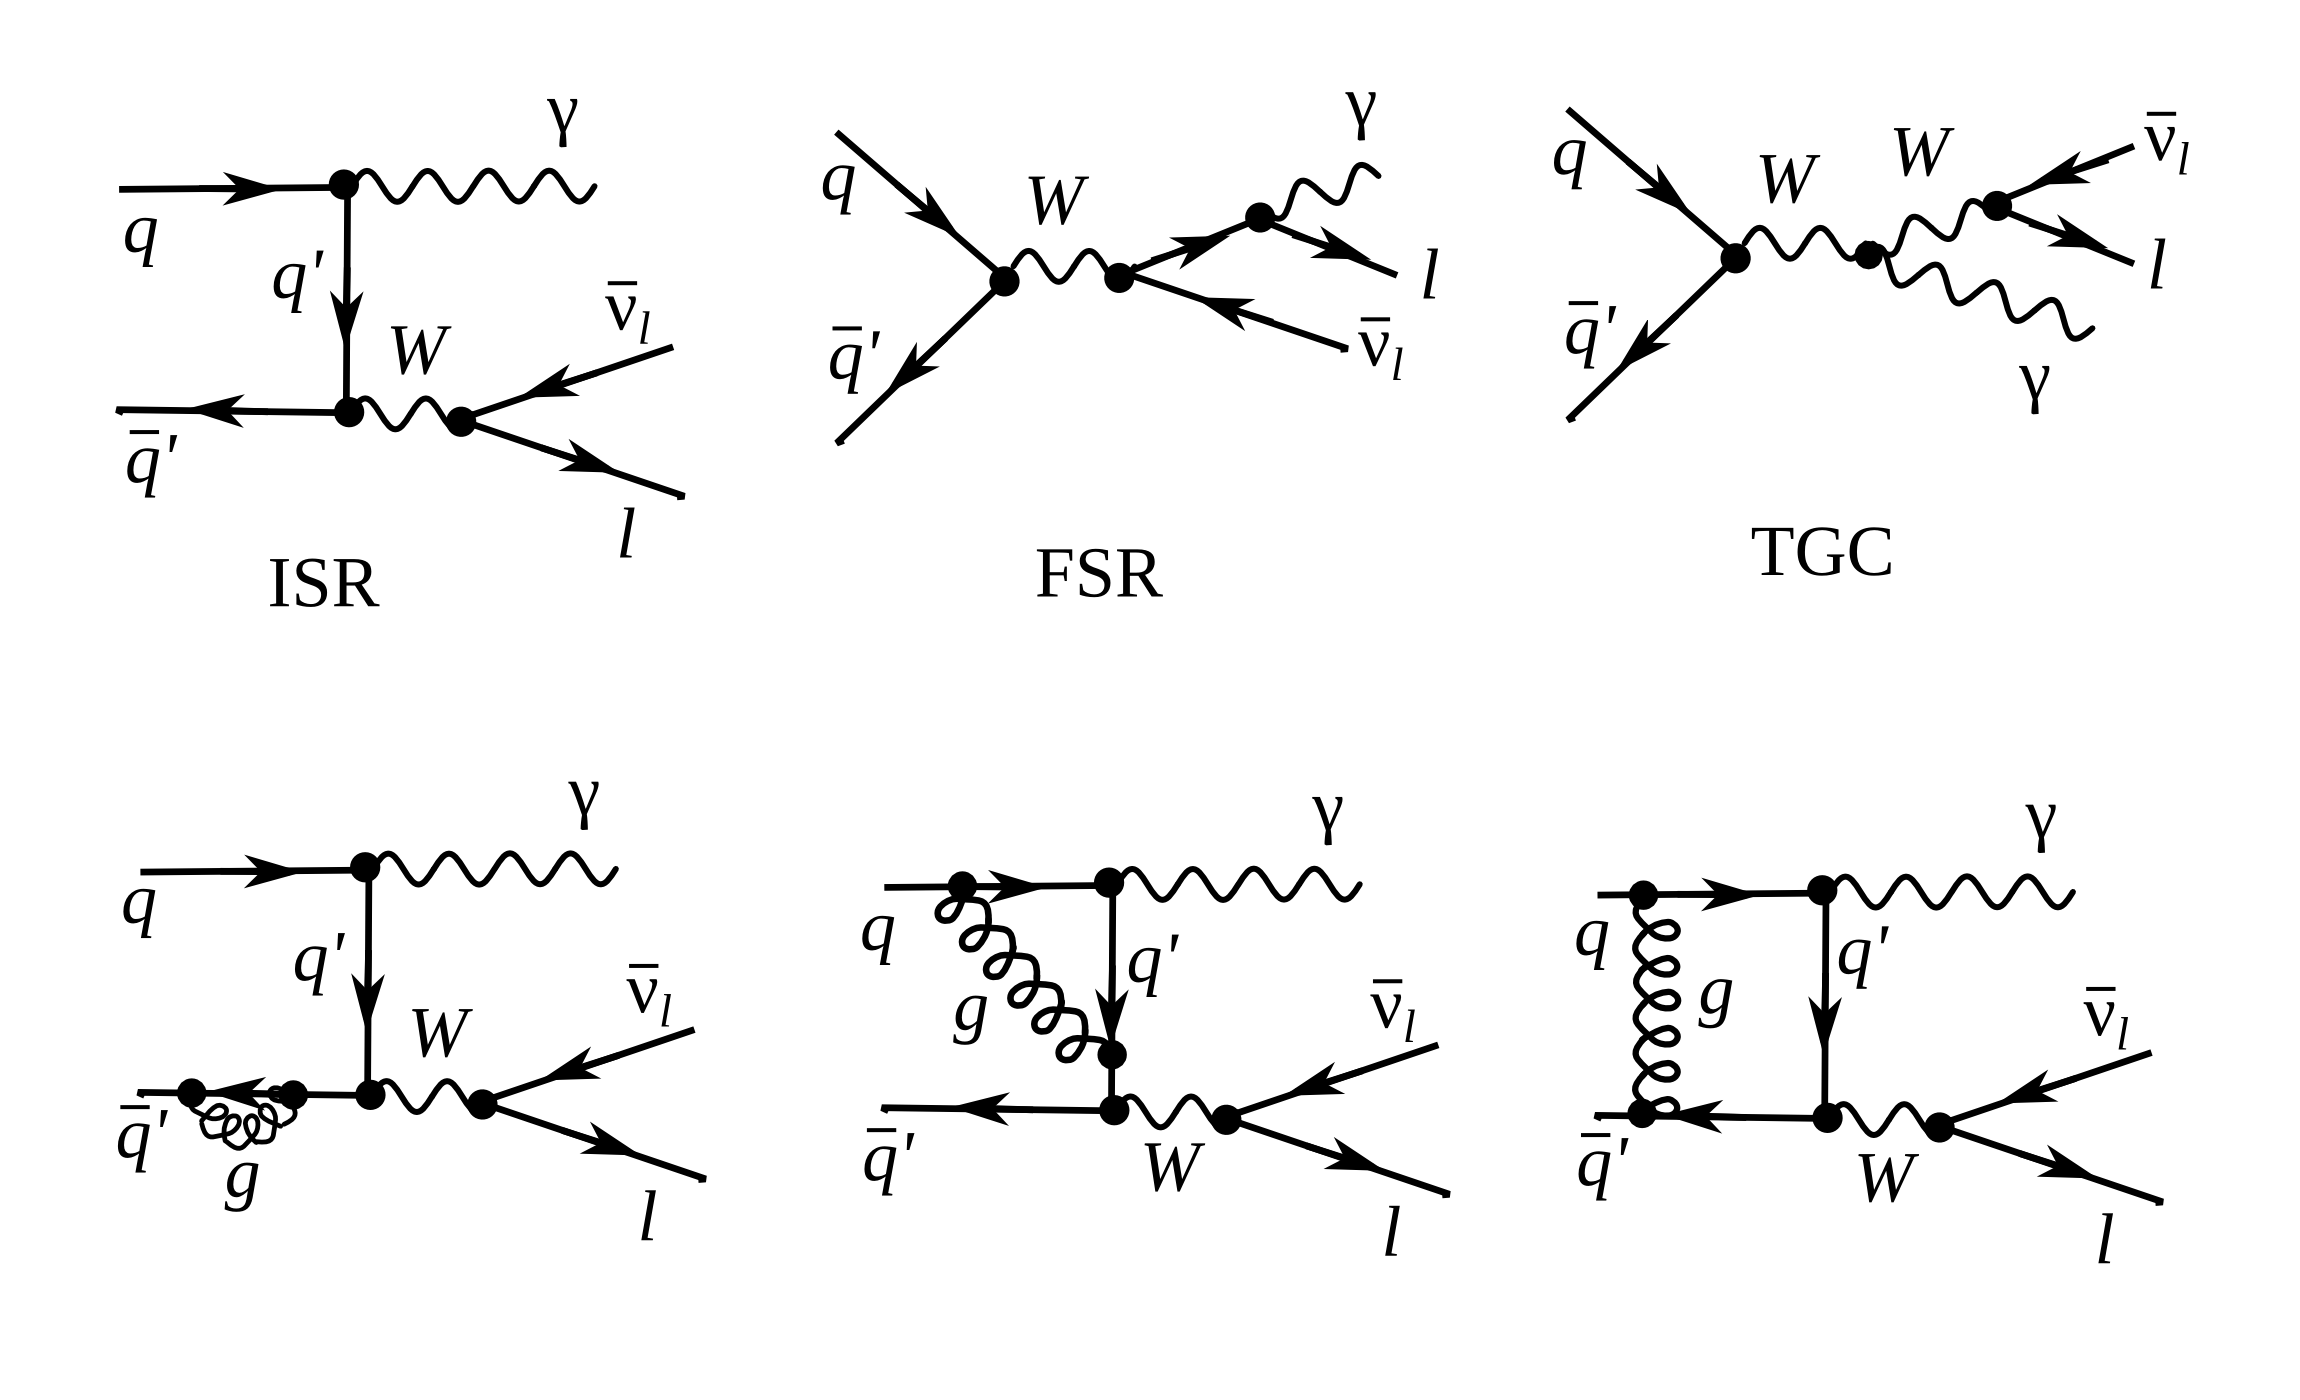
\includegraphics[width=0.90\textwidth]{../figs/WgAbout/feynmWg_LO_NLO.png}}
    \caption{Feynman diagrams of W$\gamma$ production}
    \label{fig:feynmWg_LO_NLO}
  \end{center}
\end{figure}


\begin{figure}[htb]
  \begin{center}
    {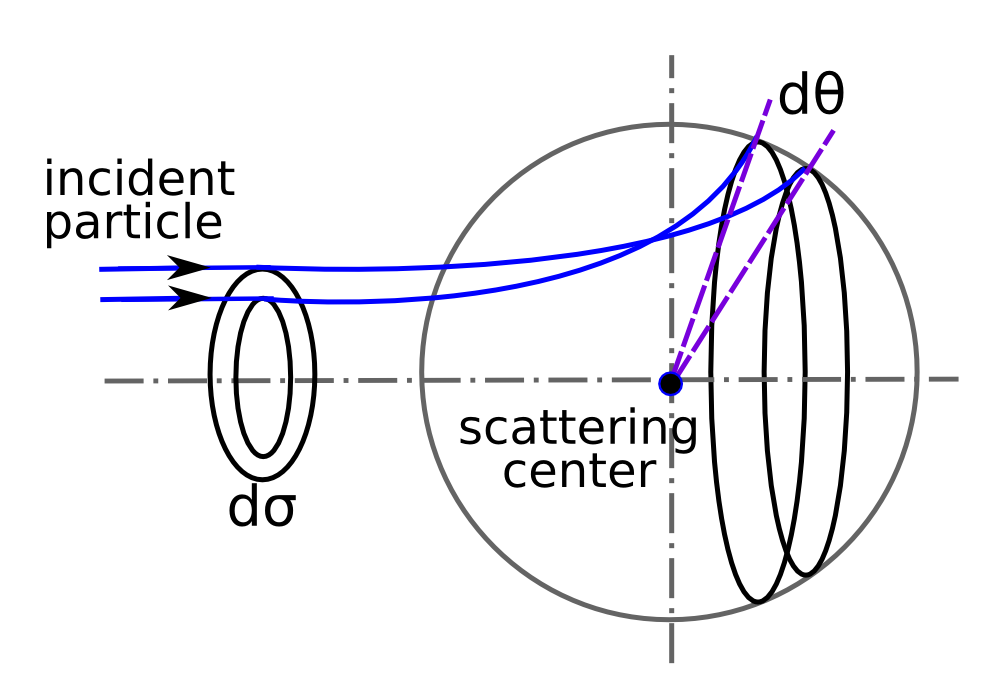
\includegraphics[width=0.70\textwidth]{../figs/WgAbout/CSclassical.png}}
    \caption{Illustration of the differential cross section concept in the classical case}
    \label{fig:CSclassical}
  \end{center}
\end{figure}

In this dissertation we are measuring the total and the differential cross section. Fig. \ref{fig:CSclassical} illustrates the concept of the differential cross section in the classical case. An incident particle must appear within area $d\sigma$ to be scattered off by an angle $d\theta$ by the scattering center. The relashionship between these two quantities would give us the expression for the differential cross section $d\sigma/d\theta$. Integrating over $d\theta$, one would get the total cross section $\sigma$. Differentiating $\sigma$ by any kinematic parameter $X$ of the incident particle would give the expression for the differential cross section $d\sigma/dX$.\\

In particle physics the cross section characterizes the probability of two particles to interact or, more specifically, the probability of two particles to interact to produce the specific final state. For example, the probability of a quark and an antiquark to interact to produce a charged lepton, a neutrino and a photon like in our measurement.\\

Referring to the Fig. \ref{fig:CSclassical}, a number of particles passing through the area $\sigma$ per unit time is $N=L \cdot \sigma$, where L is the number of particles crossing the unit area per unit time. Therefore, the cross section $\sigma$ of a specific process $\sigma=N/L$ where N is a number of events of the process occurred. $L$ in this expression refers to the number of the initial state particles and is called the luminosity. \\
  
Thus, to measure the cross section we need to know total number of events of the given process but we cannot detect events which are out of the detector acceptance or which do not fall satisfy analysis selection criteria. Therefore, the number of events $N$ has to be corrected in a measurement: $N \rightarrow N/(A \cdot \epsilon)$, where $A$ is a detector acceptance and $\epsilon$ is an efficiency of a signal process to pass selection criteria. Other corrections to $N$ may have to be applied depending on the analysis.\\

The luminosity $L$ is determined based on the collider characteristics. $L$ may not be uniform in time however we are usually interested in measuring the total or differential cross section as a function of a certain kinematic parameter of a final state particle or of a system of final state particles rather than the differential cross section as a function of time and therefore integrate the luminosity over the period of time.\\

To compute a cross section theoretically, one has to use Fermi's Golden rule. In case of the scattering of two particles to three final state particles $1+2\rightarrow 3+4+5$, it takes the following form:\\

$\sigma = \frac{ \hbar^2 }{4\sqrt{(p_1p_2)^2-(m_1m_2c^2)^2}} \int |M|^2 (2\pi)^4 \delta^4(p_1+p_2-p_3-p_4-p_5) \prod_{j=3}^{5} \frac{1}{2 \sqrt{\bar{p_j^2}+m_j^2 c^2}}\frac{d^3\bar{p_j}}{(2\pi)^3} $ \\ 
where $\hbar$ is the Planck constant, $c$ is the speed of light, $p_i$ are 4-momenta and ${\bar{p_i}}$ are three momenta of the initial state and the final state particles, $m_i$ are masses of particles, $M$ is the process amplitude.\\ 

The calculation of the process amplitude starts with writing the relevant Lagrangian similarly to how it is done in the classical mechanics but in particle physics instead of coordinates we have quantum fields. The Lagrangian allows us to derive the equations of motion however they cannot be solved exactly and, therefore, the perturbative approach is used if coupling constants are $g \ll 1$.\\

The Lagrangian term responsible for the triple gauge coupling is the following \cite{ref_theory_aTGC}:\\

$i L_{eff}^{WW\gamma}= e [ A^\mu (W_{\mu\nu}^- W^{+\nu} - W_{\mu\nu}^+ W^{-\nu}) + W_{\mu}^+ W_{\nu}^- A^{\mu\nu} ] $\\

where $e$ is the absolute value of the electron charge, $A^\mu$ is the photon field, $W^{\pm\mu}$ are fileds of $W^\pm$ bosons, $W_{\mu\nu}=\partial_\mu W_\nu - \partial_\nu W_\mu$, and $A_{\mu\nu}=\partial_\mu A_\nu - \partial_\nu A_\mu$.\\

To represent the process graphically Feynman diagrams were invented. Also the diagrams can be used to calculate the process amplitude. There is infinite number of Feynman diagrams corresponding to any specific process and the total amplitude of the process is a sum of individual amplitudes of each diagram and it is not technically possible to take into account all of them. The perturbative approach arranges all the diagrams by orders of contribution because each vertex is assigned a coupling constant and, therefore, the Feynman diagrams with fewer vertices would give a significantly larger contribution to the amplitude. In Fig. \ref{fig:feynmWg_LO_NLO} we have examples of the Leading Order (LO) and the Next-to-Leading Order (NLO) Feynman diagrams (top and bottom diagrams respectively).\\

The NLO corrections shown in Fig. \ref{fig:feynmWg_LO_NLO} are QCD corrections only which include gluon loops at the same quark line and exchange of a gluon between two different quark lines hovewer QED and weak NLO diagrams are also possible. QED corrections mean radiations of extra photons by charged particles, exchange of photons between different charged particles or a photon can be radiated and absorbed by the same charged particle forming a loop. Similarly, weak corrections mean extra virtual $W$ or $Z$ bosons. But the QCD corrections are the largest.\\

The theoretical cross section in particle physics is important not only for analysing the measurement result but also for producing the simulation which is then actively used while performing the measurement. The simulation consists of two parts: the generation of the process and the simulation of the particles paths through the detector. While the second one depends on the well-known properties of the particles and the detector configurations, the first part relies on the theory.\\  

The most precise theoretical $W\gamma$ cross section available is the NNLO cross section in QCD \cite{ref_theory_NNLO}. The effect of the NNLO correction ranges from 19\% to 26\% compared to the NLO cross section depending on the selection conditions. The contributions from the higher order corrections is estimated to be $\pm$4\%. However, the NNLO theoretical result was published in 2015 only and there is still no simulation available based on that result. The simulation used in this analisys is LO + up to two hadronic jets simulation which found to give the same predictions as the NLO result [REFERENCE to APPENDIX?].\\

In addition to the SM predictions, there are certain BSM theories which predict an enchancement of the contribution from the TGC diagram. The discussion of these BSM effects on the $W\gamma$ process takes place in chapter \ref{sec:WgAbout_ATGC}.\\ 


